\begin{figure}[H]
    \centering
    \begin{adjustbox}{width=12cm,center}
    \frame{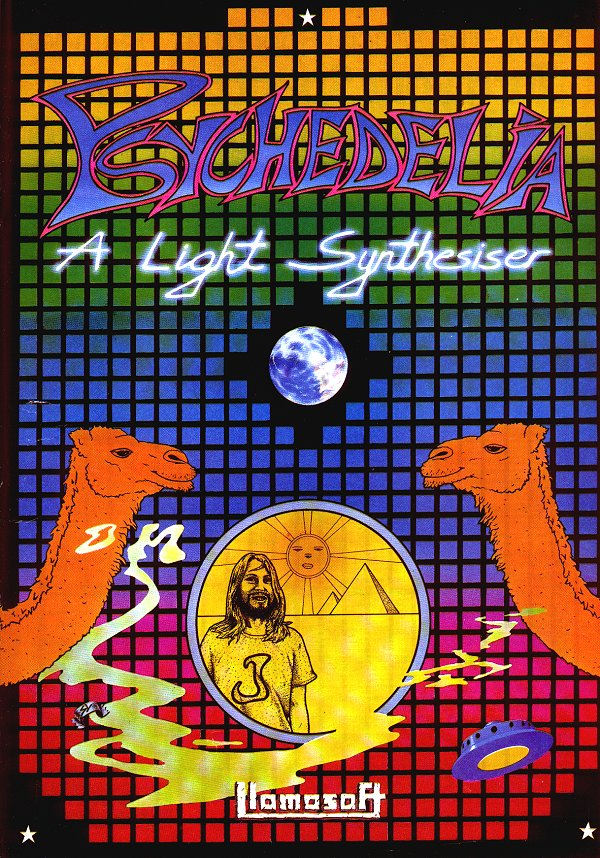
\includegraphics{src/preface/psychedelia.jpg}}%
    \end{adjustbox}
\caption{Cover art by Steinar Lund for the commercial edition of Psychedelia}
\end{figure}
\clearpage
\chapter*{about this book} 
This is a book about a toy. A toy that was the first of its kind. A kind of toy that has never really caught on,
though maybe its moment lies some way in the future. 

A static picture does the toy no justice, but we will show a few anyway. If you do not know what Psychedelia is, they
might at least give you a flavour of this game that is not a game. 
\begin{figure}[H]
    \begin{adjustbox}{width=10cm,center}
    \frame{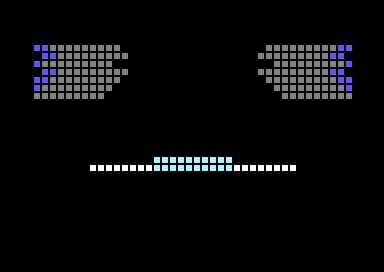
\includegraphics{src/preface/p1.png}}%
      \hspace{0.1cm}
    \frame{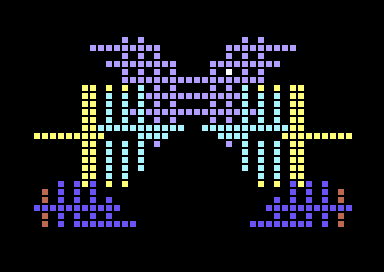
\includegraphics{src/preface/p2.png}}%
    \end{adjustbox}
\end{figure}
\vspace{-0.8cm}
\begin{figure}[H]
    \begin{adjustbox}{width=10cm,center}
    \frame{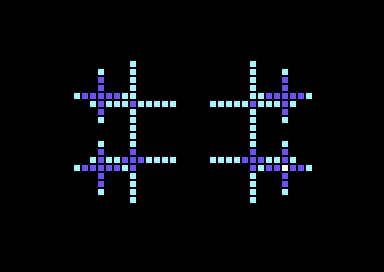
\includegraphics{src/preface/p3.png}}%
      \hspace{0.1cm}
    \frame{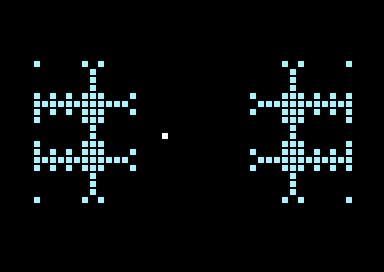
\includegraphics{src/preface/p4.png}}%
    \end{adjustbox}
\end{figure}

Rob Hogan (\href{https://mastodon.social/@mwenge}{\textcolor{blue}{@mwenge}})\\
Dublin \the\year{} \\

\clearpage
\vspace*{\fill}
\begin{figure}[H]
    \centering
      
\includegraphics[width=5cm]{src/cover/title_page.png}%
\end{figure}
\vspace*{\fill}
\thispagestyle{empty}%
\clearpage

